\chapter{O átomo de hidrogênio}\label{ch:b3:hydrogen-atom}

Nove décimos dos átomos do universo são hidrogênio: um próton que
segura um elétron, o único átomo que a física resolve exatamente --- e
a chave que abriu todos os outros. A velha teoria quântica do
\cref{ch:b3:hamiltonian-mechanics} adivinhou suas energias; a
maquinaria está agora pronta para \emph{deduzi-las}: o potencial de
Coulomb entra na \omterm{prop:b3:schrodinger-three-dimensions:swave}{equação radial} do capítulo anterior, e de lá saem os
níveis $-E_{\text{I}}/n^2$, o \omterm{thm:b3:hydrogen-atom:levels}{raio de Bohr}, as camadas e subcamadas da
tabela periódica da química e as séries espectrais que os astrônomos
leem em toda nebulosa. A mesma solução, reescalada, descreve o hélio
ionizado, os átomos muônicos, o positrônio e os ``átomos'' de par
elétron--buraco dentro dos semicondutores; esticada até $n
\approx 100$, ela descreve átomos de Rydberg de meio micrômetro de
diâmetro, cujos sussurros de rádio mapeiam as nuvens ionizadas da
Galáxia e cujas interações hoje movem computadores quânticos.
% NOTE: full radial solutions (Laguerre) admitted; ground state solved
% exactly; emphasis on scaling laws and applications.

\section{O problema de Coulomb resolvido}

\begin{theorem}[Níveis do hidrogênio]\label{thm:b3:hydrogen-atom:levels}
\index{átomo de hidrogênio}\index{número quântico principal}\index{raio de Bohr}
Para $V(r) = -e^2/4\pi\varepsilon_0 r$ (escreva $k = e^2/4\pi
\varepsilon_0$), os estados ligados são rotulados por $(n, l, m)$ com
\[
E_n = -\frac{E_{\text{I}}}{n^2} , \qquad
E_{\text{I}} = \frac{m_{\text{e}}k^2}{2\hbar^2} = \qty{13.6}{eV} ,
\qquad n = 1, 2, 3, \dots
\]
e, para cada $n$, os números orbitais $l = 0, 1, \dots, n-1$ e
$m = -l, \dots, l$. O comprimento natural é o \omterm{thm:b3:hydrogen-atom:levels}{raio de Bohr} $a_0 =
\hbar^2/m_{\text{e}}k = \qty{52.9}{pm}$; o estado fundamental é
\[
\psi_{100} = \frac{1}{\sqrt{\pi a_0^3}}\;\eu^{-r/a_0} .
\]
A energia depende \emph{apenas} de $n$: contando os $m$ e os $l$, o
nível $n$ tem degenerescência $n^2$ (dobrada pelo spin,
\cref{ch:b3:spin-two-level}) --- muito além da degenerescência
$(2l+1)$ que a isotropia explica.
\end{theorem}

\begin{proof}[Demonstração parcial]
Para o estado fundamental, tente $u = Cr\,\eu^{-r/a}$ na \omterm{prop:b3:schrodinger-three-dimensions:swave}{equação radial}
com $l = 0$: $u'' = (1/a^2 - 2/ar)u$, de modo que
$-\tfrac{\hbar^2}{2m_{\text{e}}}u'' - \tfrac kr u = Eu$ exige
$\hbar^2/m_{\text{e}}a = k$ (igualando os termos em $1/r$) --- o que é
$a = a_0$ --- e $E = -\hbar^2/2m_{\text{e}}a_0^2 = -E_{\text{I}}$. A
solução geral (polinômios de Laguerre, com $n - l - 1$ nós radiais) é
admitida; cada passo da construção é elementar, mas longo. A
degenerescência ``acidental'' em $l$ espelha um segredo clássico da
força $1/r$ pura --- as elipses de Kepler não precessam, e um vetor
conservado a mais (Laplace--Runge--Lenz) aponta ao longo do eixo maior
fixo; sua versão quântica é o que amarra diferentes $l$ a uma mesma
energia (\cref{exo:b3:hydrogen-atom:12}).
\end{proof}

\begin{omfigure}
\begin{tikzpicture}[font=\small, >=Stealth]
  % energy scale: E = -13.6/n^2, map E -> y = 5.6 + E*0.42 (E in eV)
  % n=1: y=-0.11? choose y(E) = 5.9 + 0.42*E: n1: 0.19, n2: 4.47, n3: 5.27, n4: 5.55, inf: 5.9
  \draw[->] (-0.4,-0.4) -- (-0.4,6.6);
  \node[anchor=south] at (-0.4,6.6) {$E$ (eV)};
  % continuum
  \fill[gray!15] (0,5.9) rectangle (8.6,6.45);
  \node[anchor=west, font=\footnotesize] at (8.7,6.15) {contínuo: ionizado};
  \draw[thick] (0,5.9) -- (8.6,5.9);
  \node[anchor=east, font=\footnotesize] at (-0.5,5.9) {$0$};
  % levels, split by l columns
  \foreach \n/\y in {1/0.19, 2/4.47, 3/5.27, 4/5.55}
    {\node[anchor=east, font=\footnotesize] at (-0.5,\y) {$-13.6/\n^2$};}
  % l columns: s at x 0-1.4, p at 1.9-3.3, d at 3.8-5.2, f 5.7-7.1
  \node[font=\footnotesize] at (0.7,-0.3) {$l = 0$ ($s$)};
  \node[font=\footnotesize] at (2.6,-0.3) {$l = 1$ ($p$)};
  \node[font=\footnotesize] at (4.5,-0.3) {$l = 2$ ($d$)};
  \node[font=\footnotesize] at (6.4,-0.3) {$l = 3$ ($f$)};
  \draw[very thick, omDef] (0,0.19) -- (1.4,0.19);
  \foreach \x in {0,1.9} \draw[very thick, omDef] (\x,4.47) -- ({\x+1.4},4.47);
  \foreach \x in {0,1.9,3.8} \draw[very thick, omDef] (\x,5.27) -- ({\x+1.4},5.27);
  \foreach \x in {0,1.9,3.8,5.7} \draw[very thick, omDef] (\x,5.55) -- ({\x+1.4},5.55);
  % series arrows
  \draw[->, omExo, thick] (0.5,4.47) -- (0.6,0.24);
  \draw[->, omExo, thick] (1.0,5.27) -- (0.85,0.24);
  \node[omExo, font=\footnotesize, anchor=west] at (0.95,2.3) {Lyman (UV)};
  \draw[->, omThm, thick] (2.6,5.27) -- (2.45,4.52);
  \draw[->, omThm, thick] (3.1,5.55) -- (2.9,4.52);
  \node[omThm, font=\footnotesize, anchor=west] at (3.25,4.95) {Balmer (visível)};
  \node at (1.9,1.55) {};
\end{tikzpicture}

{\small Os níveis do hidrogênio $-E_{\text{I}}/n^2$, distribuídos por
$l$: todas as subcamadas de um mesmo $n$ coincidem (o ``acidente'' de
Coulomb). Os saltos para baixo que terminam em $n = 1$ formam a série
ultravioleta de Lyman; os que terminam em $n = 2$, a série visível de
Balmer, que tinge as nebulosas de vermelho.}
\end{omfigure}

\section{Onde está o elétron}

\begin{proposition}[Distribuições radiais]\label{prop:b3:hydrogen-atom:radial}
\index{probabilidade radial}
A probabilidade de encontrar o elétron entre $r$ e $r + \dd r$ vale
$P(r)\,\dd r$, com $P(r) = |u(r)|^2$, o quadrado da função radial
normalizada do \cref{thm:b3:quantum-angular-momentum:radial}. Para os estados mais baixos:
$P_{1s} \propto r^2\eu^{-2r/a_0}$, com pico exatamente em $r = a_0$ e
$\langle r\rangle = \tfrac32 a_0$; $P_{2s}$ mostra duas corcovas
separadas por um \emph{nó} esférico; $P_{2p} \propto
r^4\eu^{-r/a_0}$, com pico em $4a_0$. Em geral, $\langle r\rangle
\approx n^2a_0$: os átomos crescem \emph{quadraticamente} com a
excitação, enquanto sua ligação encolhe como $1/n^2$ --- a alavanca por
trás dos gigantes de Rydberg do \cref{pb:b3:hydrogen-atom:1}.
\end{proposition}
\admitted

\begin{omfigure}
\begin{tikzpicture}
  \begin{axis}[omaxis, axis x line=bottom, axis y line=left,
    width=11.6cm, height=5.8cm, xmin=0, xmax=14, ymin=0, ymax=0.62,
    xlabel={$r/a_0$}, ylabel={$P(r)$ (por $a_0$)},
    xlabel style={at={(axis description cs:0.5,-0.1)}, anchor=north},
    xtick={1,4,5,10}, ytick=\empty, clip=false,
    legend style={font=\scriptsize, at={(0.95,0.9)}, anchor=north east,
      draw=none, fill=none}]
    \addplot[omDef, very thick, domain=0:8, samples=120] {4*x*x*exp(-2*x)};
    \addlegendentry{$1s$}
    \addplot[omThm, thick, domain=0:14, samples=140] {0.125*x*x*(2-x)^2*exp(-x)};
    \addlegendentry{$2s$}
    \addplot[omExo, thick, domain=0:14, samples=140] {x^4*exp(-x)/24};
    \addlegendentry{$2p$}
    \draw[gray, dashed] (axis cs:1,0) -- (axis cs:1,0.545);
  \end{axis}
\end{tikzpicture}

{\small Densidades de \omterm{prop:b3:hydrogen-atom:radial}{probabilidade radial}. O pico do $1s$ fica
exatamente em $a_0$; o estado $2s$ carrega um nó esférico e um lóbulo
perto do núcleo --- a ``penetração'' que ordenará a tabela periódica
--- ao passo que o $2p$, murado pela \omterm{thm:b3:quantum-angular-momentum:radial}{barreira centrífuga}, mantém
distância.}
\end{omfigure}

\begin{example}[Ler os tamanhos]\label{ex:b3:hydrogen-atom:sizes}
Estado fundamental: \qty{0.1}{nm} de diâmetro, \qty{13.6}{eV} de
profundidade --- as escalas de toda a química. Em $n = 10$: raio
$\sim\qty{5}{nm}$, ligação de \qty{0.136}{eV} --- frouxamente preso. Em
$n = 100$: um átomo de escala \emph{micrométrica} ligado por
\qty{1.4}{meV}, destruído pelo mais débil dos campos --- e, ainda
assim, o espaço interestelar é vazio o bastante para que tais átomos
vivam e transmitam (\cref{pb:b3:hydrogen-atom:1}).
\end{example}

\section{O espectro}

\begin{proposition}[Séries e regras de seleção]\label{prop:b3:hydrogen-atom:series}
\index{série de Balmer}\index{série de Lyman}
Um salto $n' \to n$ emite o comprimento de onda
\[
\frac{1}{\lambda} = R_{\text{H}}\Big(\frac{1}{n^2} -
\frac{1}{n'^2}\Big) , \qquad
R_{\text{H}} = \frac{E_{\text{I}}}{hc} = \qty{1.097e7}{m^{-1}} ,
\]
sujeito à regra de seleção dipolar $\Delta l = \pm1$ (o fóton carrega
$\hbar$). A \omterm{prop:b3:hydrogen-atom:series}{série de Lyman} ($\to n = 1$) fica no ultravioleta distante,
a partir de \qty{121.6}{nm}; a \omterm{prop:b3:hydrogen-atom:series}{série de Balmer} ($\to n = 2$) começa na
linha vermelha $H\alpha$, em \qty{656.3}{nm} --- a cor das nebulosas de
emissão e das proeminências solares; as séries de Paschen e seguintes
recuam para o infravermelho e, entre $n = 110$ e $109$, a mesma fórmula
aterrissa em \qty{5.0}{GHz}: o hidrogênio fala do ultravioleta ao dial
do rádio.
\end{proposition}

\begin{proof}
Conservação de energia com o \cref{thm:b3:hydrogen-atom:levels};
$R_{\text{H}}$ como no \cref{pb:b3:hamiltonian-mechanics:1}, agora
deduzido em vez de postulado.
\end{proof}

\begin{example}[Átomos hidrogenoides: uma solução, muitos átomos]\label{ex:b3:hydrogen-atom:scaling}
Substitua a carga do próton por $Ze$ e o elétron por qualquer massa
$\mu$ em órbita: toda fórmula se reescala como
\[
a \to a_0\,\frac{m_{\text{e}}}{\mu}\,\frac1Z , \qquad
E_{\text{I}} \to E_{\text{I}}\,\frac{\mu}{m_{\text{e}}}\,Z^2 .
\]
He$^+$ ($Z = 2$): \qty{54.4}{eV}. Elétrons internos de átomos pesados
($Z \sim 30$): energias da camada K na faixa do keV --- os raios X
característicos com que Moseley ordenou os elementos
(\cref{exo:b3:hydrogen-atom:5}). Hidrogênio muônico ($\mu = 207
m_{\text{e}}$): um átomo de escala femtométrica que sonda o próprio
próton. Positrônio ($e^+e^-$, $\mu = m_{\text{e}}/2$): metade da
ligação, o dobro do tamanho e uma vida curta que termina em fótons de
aniquilação. E, num semicondutor, um elétron e um buraco orbitam um ao
outro com massas efetivas pequenas num dielétrico que blinda a
interação: um \emph{éxciton}, o mesmo átomo crescido até dez nanômetros
e milielétron-volts (\cref{exo:b3:hydrogen-atom:7}) --- o hidrogênio é
menos um átomo do que um molde.
\end{example}

\begin{omfigure}
\begin{tikzpicture}[font=\small]
  % size comparison, hand-drawn
  \draw[omDef, thick, fill=omDef!12] (1.2,0) circle (1.05);
  \fill[omDef] (1.2,0) circle (1.5pt);
  \node[align=center, font=\footnotesize] at (1.2,-1.75)
    {hidrogênio\\$a_0$, \qty{-13.6}{eV}};
  \draw[omThm, thick, fill=omThm!12] (4.6,0) circle (0.42);
  \fill[omThm] (4.6,0) circle (1.5pt);
  \node[align=center, font=\footnotesize] at (4.6,-1.75)
    {H muônico\\$a_0/207$ ($\times 40$ aqui)\\\qty{-2.5}{keV}};
  \draw[omExo, thick, fill=omExo!12] (8.1,0) circle (1.55);
  \fill[omExo] (8.1,0) circle (1.5pt);
  \node[align=center, font=\footnotesize] at (8.1,-2.25)
    {positrônio\\$2a_0$, \qty{-6.8}{eV}};
  \draw[omProp, thick, fill=omProp!10] (12.4,0) circle (2.0);
  \fill[omProp] (12.4,0) circle (1.5pt);
  \node[align=center, font=\footnotesize] at (12.4,-2.75)
    {éxciton num cristal\\$\sim 170\,a_0$ ($\div 50$ aqui)\\$\sim\qty{-7}{meV}$};
\end{tikzpicture}

{\small Uma solução, quatro ``átomos'': reescalar massa, carga e
vizinhança dielétrica transforma o hidrogênio em sondas do próton, em
testes de eletrodinâmica quântica pura e nos quase átomos emissores de
luz dos semicondutores.}
\end{omfigure}

\begin{method}[Trabalhar com sistemas hidrogenoides]\label{met:b3:hydrogen-atom:method}
(1) Reescale primeiro: $a \propto 1/\mu Z$ e $E \propto \mu Z^2$
transformam qualquer resposta do hidrogênio em qualquer resposta
hidrogenoide. (2) Tamanhos: $\langle
r\rangle \sim n^2a$; espaçamentos perto do nível $n$: $\dd E/\dd n =
2E_{\text{I}}/n^3$. (3) Espectros: fórmula de Rydberg mais
$\Delta l =
\pm1$. (4) Penetração: os estados $s$ sentem o núcleo, os
de $l$ alto orbitam por fora --- a alavanca da química de vários
elétrons. (5) Âncoras de sanidade: $\qty{13.6}{eV}$, $\qty{52.9}{pm}$,
$\qty{121.6}{nm}$ e $\qty{656.3}{nm}$ --- quatro números que vale a
pena memorizar para a vida toda.
\end{method}

\begin{omfigure}
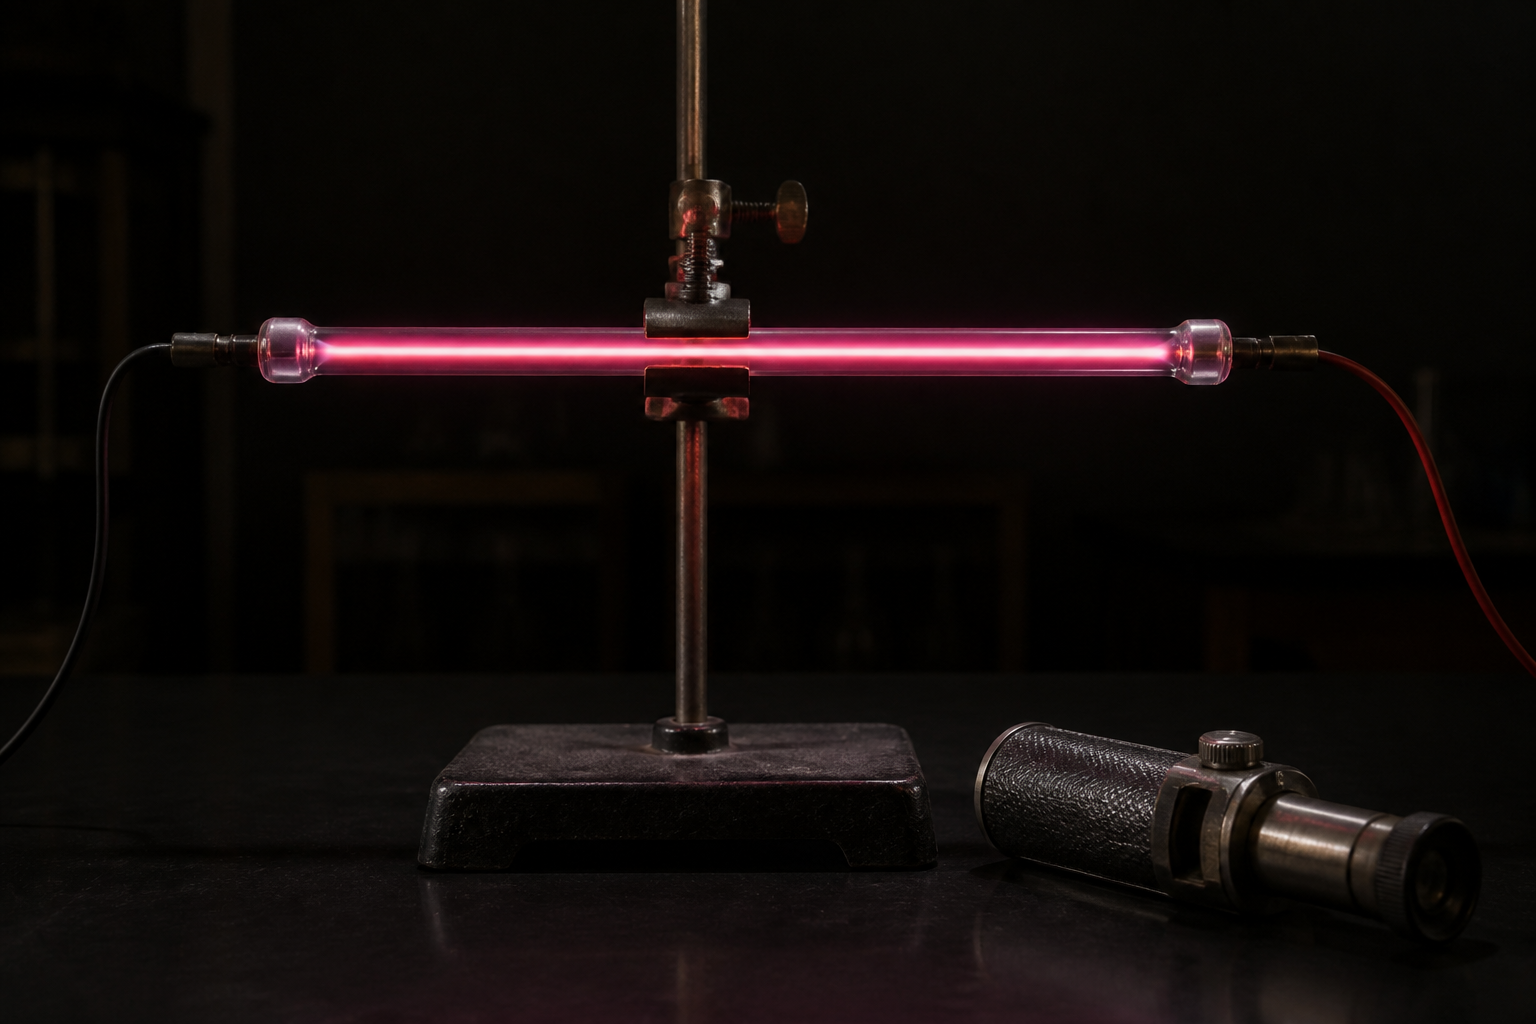
\includegraphics[width=0.58\linewidth]{images/book5/ai/b5-11-discharge-tube.png}

{\small Um tubo de descarga de hidrogênio e um espectroscópio de bolso: o brilho rosado, decomposto, torna-se as linhas de Balmer --- a impressão digital inteira que este capítulo deduz do potencial de Coulomb.}
\end{omfigure}

\section{Exercícios}

\begin{exercise}[$\star$]\label{exo:b3:hydrogen-atom:1}
(a) Verifique por substituição que $u = Cr\eu^{-r/a_0}$ resolve a
\omterm{prop:b3:schrodinger-three-dimensions:swave}{equação radial} de $l = 0$ com $E = -E_{\text{I}}$, desde que $a_0 =
\hbar^2/m_{\text{e}}k$. (b) Normalize-a ($\int_0^\infty
x^2\eu^{-x}\dd x = 2$). (c) Confira as dimensões de $a_0$ e de
$E_{\text{I}}$. (d) Por que não existe estado abaixo de $-E_{\text{I}}$
(argumente com o \cref{exo:b3:schrodinger-three-dimensions:12})?
\end{exercise}

\begin{exercise}[$\star$]\label{exo:b3:hydrogen-atom:2}
Calcule (a) os comprimentos de onda da Lyman $\alpha$ e do limite de
Lyman; (b) as três primeiras linhas de Balmer e o limite de Balmer ---
quais são visíveis, e de que cores? (c) a faixa da série de Paschen;
(d) a frequência da transição $n = 110 \to 109$.
\end{exercise}

\begin{exercise}[$\star$]\label{exo:b3:hydrogen-atom:3}
Para o estado fundamental: (a) localize o máximo de $P_{1s}(r)$; (b)
calcule $\langle r\rangle$; (c) calcule a probabilidade de encontrar o
elétron além de $2a_0$ ($\int_x^\infty t^2\eu^{-t}\dd t = (x^2 +
2x + 2)\eu^{-x}$); (d) por que as imagens de ``órbita'' de raio
exatamente $a_0$ enganam?
\end{exercise}

\begin{exercise}[$\star$]\label{exo:b3:hydrogen-atom:4}
(a) Liste os pares $(l, m)$ de $n = 3$ e verifique a contagem $n^2 =
9$. (b) Com o spin, quantos estados há nas camadas $n = 1, 2, 3$? (c)
Relacione-os com os comprimentos $2, 8, 18$ das linhas da tabela
periódica. (d) Que degenerescência (em $m$ ou em $l$) sobrevive no
elétron externo do sódio, e por que a outra se quebra?
\end{exercise}

\begin{exercise}[$\star\star$]\label{exo:b3:hydrogen-atom:5}
A escada de Moseley. Um elétron interno (da camada K) de um elemento
$Z$ se move num campo nuclear quase nu, blindado pelo único outro
elétron K: carga efetiva $\approx Z - 1$. (a) Mostre que a energia do
raio X $2p \to 1s$ vale aproximadamente
$\tfrac34(Z-1)^2E_{\text{I}}$. (b) Avalie-a para o cobre ($Z = 29$) e
compare com a K$\alpha$ medida em \qty{8.05}{keV}. (c) Moseley (1913)
traçou $\sqrt{\nu}$ contra $Z$ e obteve retas: o que isso provou sobre
o significado do número atômico? (d) Preveja a energia K$\alpha$ do
elemento $Z = 43$, então faltante.
\end{exercise}

\begin{exercise}[$\star\star$]\label{exo:b3:hydrogen-atom:6}
Positrônio. (a) Justifique $\mu = m_{\text{e}}/2$ e dê sua energia de
ligação e seu \omterm{thm:b3:hydrogen-atom:levels}{raio de Bohr}. (b) Seu comprimento de onda Lyman $\alpha$.
(c) O para-positrônio se aniquila em dois fótons: as energias deles e
as direções relativas (a partir do
\cref{ch:b3:relativistic-dynamics}). (d) Onde a medicina detecta
exatamente essa assinatura todos os dias?
\end{exercise}

\begin{exercise}[$\star\star$]\label{exo:b3:hydrogen-atom:7}
Éxcitons. No arseneto de gálio, $\varepsilon_{\text{r}} = 12.9$ e a
massa efetiva reduzida vale $\mu = 0.058\,m_{\text{e}}$. (a) Mostre que
$a_{\text{ex}} = a_0\,\varepsilon_{\text{r}}\,m_{\text{e}}/\mu$ e
avalie. (b) A energia de ligação do éxciton. (c) Compare
$a_{\text{ex}}$ com os raios dos pontos quânticos do
\cref{pb:b3:schrodinger-three-dimensions:1} e justifique, enfim, o
descarte do termo de Coulomb em pontos pequenos. (d) Por que as linhas
excitônicas só aparecem em semicondutores \emph{puros e frios}
($k_{\text{B}}T$ contra a sua resposta de (b))?
\end{exercise}

\begin{exercise}[$\star\star$]\label{exo:b3:hydrogen-atom:8}
Penetração e os metais alcalinos. O sódio é um elétron de valência
hidrogenoide fora de um caroço fechado de carga efetiva $+e$.
(a) Qual dos estados $3s$, $3p$, $3d$ sente mais o núcleo
incompletamente blindado, e por quê (lembre a figura radial)? (b) Os
níveis medidos são $E_{3s} = \qty{-5.14}{eV}$, $E_{3p} = \qty{-3.04}{eV},
E_{3d} = \qty{-1.52}{eV}$: verifique que o $3d$ é quase hidrogenoide
($n = 3$), enquanto o $3s$ é bem mais profundo, e explique. (c) Calcule
o comprimento de onda de $3p \to 3s$: que cor famosa é essa? (d)
Escreva os níveis alcalinos como $-E_{\text{I}}/(n - \delta_l)^2$ e
extraia os ``defeitos quânticos'' $\delta_s$ e $\delta_p$ do sódio.
\end{exercise}

\begin{exercise}[$\star\star$]\label{exo:b3:hydrogen-atom:9}
Um próton numa nebulosa captura um elétron em $n = 100$. (a) Quanta
energia é liberada no fóton de captura, se o elétron chegou quase
livre? (b) O átomo desce em cascata, preferencialmente por passos
$\Delta n = 1$ em $n$ alto: em que faixa caem esses fótons? (c) O
último passo da cascata é a Lyman $\alpha$; a luz visível das nebulosas
é dominada pela H$\alpha$: identifique que passo da cascata é esse. (d)
Explique por que as nebulosas de emissão brilham em \emph{vermelho},
embora a linha mais forte do hidrogênio (a Lyman $\alpha$) seja
ultravioleta.
\end{exercise}

\begin{exercise}[$\star\star\star$]\label{exo:b3:hydrogen-atom:10}
Médias e o virial. Para o estado fundamental, calcule (a)
$\langle 1/r\rangle$ e verifique $\langle E_p\rangle = -2E_{\text{I}}
= 2E_1$; (b) $\langle E_k\rangle = +E_{\text{I}}$, confirmando a razão
do virial do \cref{exo:b3:hamiltonian-mechanics:4}; (c) a velocidade
quadrática média do elétron e $v/c$; (d) a ordem de grandeza do campo magnético que o
\emph{próton} sente por causa do movimento do elétron (uma espira de
corrente $ev/2\pi a_0$ vista à distância $a_0$) --- um número de que a
estrutura hiperfina precisará.
\end{exercise}

\begin{exercise}[$\star\star\star$]\label{exo:b3:hydrogen-atom:11}
Quão fina é a estrutura fina. (a) Mostre que a escala de velocidade do
estado fundamental é $\langle v^2\rangle^{1/2}/c = \alpha \approx 1/137$
e que, para um hidrogenoide de $Z$, ela vale $Z\alpha/n$. (b) As
correções relativísticas entram em ordem relativa $(v/c)^2$: estime a
escala de estrutura fina $\alpha^2E_{\text{I}}$ em meV e a ordem do
desdobramento para $n = 2$ em GHz. (c) Para o urânio hidrogenoide
($Z = 92$): $v/c$ em $n = 1$ --- o tratamento não relativístico se
sustenta? (d) O que a divergência formal em $Z\alpha \to 1$
($Z \approx 137$) anuncia fisicamente?
\end{exercise}

\begin{exercise}[$\star\star\star$]\label{exo:b3:hydrogen-atom:12}
A degenerescência desarrazoada. (a) Na mecânica clássica, mostre que,
para $V = -k/r$, a órbita se fecha (sem precessão), citando o vetor
conservado de Laplace--Runge--Lenz $\vect A = \vect p\wedge\vect
L - mk\,\vect e_r$ --- verifique $\dd\vect A/\dd t = 0$ usando a lei de
Newton. (b) Argumente: um vetor conservado que fixa o eixo da elipse é
uma simetria a mais, além das rotações --- e simetria a mais significa
degenerescência a mais (lembre o \cref{exo:b3:quantum-formalism:9}).
(c) Acrescente uma pequena correção em $1/r^2$ ao potencial e mostre
que a elipse precessa: o eixo gira e $\vect A$ deixa de se conservar.
(d) Conecte: nos átomos de vários elétrons, o potencial efetivo não é
$1/r$ puro, e a degenerescência em $l$ se quebra (o sódio!); no próprio
hidrogênio, é a relatividade que fornece a pequena correção --- que
característica observada do \cref{exo:b3:hydrogen-atom:11} é essa?
\end{exercise}

\section{Problema: Átomos gigantes}

\begin{problem}[{Problema de fim de semana --- átomos de Rydberg, do
brilho de rádio da Galáxia aos computadores quânticos}]\label{pb:b3:hydrogen-atom:1}
Estique o hidrogênio até $n \approx 100$ e ele se torna um objeto de
outra espécie: micrômetros de diâmetro, ligado por milielétron-volts,
absurdamente sensível --- e absurdamente útil. Este problema amplia a
solução do hidrogênio, primeiro até as nuvens interestelares que
transmitem em comprimentos de onda centimétricos, depois até os
arranjos de laboratório em que tais gigantes se emaranham uns nos
outros e formam processadores. Dados:
$E_{\text{I}} = \qty{13.6}{eV}$, $a_0 = \qty{52.9}{pm}$,
$R_{\text{H}}c = \qty{3.29e15}{Hz}$, e o $k_{\text{B}}T$ a
\qty{300}{K} vale \qty{25.9}{meV}.

\medskip\noindent\textbf{Parte I --- As leis de escala.}
\begin{enumerate}
  \item Dê as quatro escalas básicas com $n$: o tamanho $\langle
        r\rangle$, a ligação $|E_n|$, o espaçamento $E_{n+1} - E_n$
        (para $n$ grande) e a frequência orbital clássica da órbita de
        Bohr correspondente.
  \item Mostre que, para $n$ grande, a frequência de transição $n+1 \to
        n$ se aproxima de $2R_{\text{H}}c/n^3$ e verifique
        que ela é igual à frequência orbital clássica (o princípio da
        correspondência do \cref{pb:b3:hamiltonian-mechanics:1},
        completado).
  \item Avalie o tamanho e a ligação em $n = 50$ e $n = 100$.
  \item O dipolo elétrico de um átomo de Rydberg escala como $n^2ea_0$:
        avalie-o em $n = 50$, em debyes ($1\,\text{D} =
        \qty{3.34e-30}{C.m}$), e compare com os \qty{1.85}{D} de uma
        molécula de água.
  \item Estime o campo elétrico que despedaça o átomo de $n = 50$,
        como $F \sim |E_n|/(e\,\langle r\rangle)$, em V/cm.
  \item Por que átomos assim não sobrevivem à química ordinária do
        vácuo de laboratório --- e, no entanto, sobrevivem muito bem no
        espaço interestelar (compare as taxas de colisão)?
\end{enumerate}

\medskip\noindent\textbf{Parte II --- As linhas de recombinação da
Galáxia.}
Nas nebulosas ionizadas, os prótons capturam elétrons em $n$ alto; a
cascata irradia um pente de ``linhas de recombinação de rádio''.
\begin{enumerate}[resume]
  \item Calcule a frequência da transição $n = 110 \to 109$
        (chamada H109$\alpha$).
  \item Em que faixa ela cai, e que tipo de telescópio a recebe?
  \item Calcule o comprimento de onda da H109$\alpha$ e compare-o com
        o tamanho do átomo emissor: quantos átomos cabem num
        comprimento de onda?
  \item Essas linhas medem a temperatura da nebulosa por sua largura
        Doppler: a $T = \qty{e4}{K}$, a velocidade térmica do
        hidrogênio é $\sim\qty{12.8}{km/s}$ --- calcule a largura
        relativa de linha $\Delta\nu/\nu$ e a largura da H109$\alpha$
        em kHz.
  \item As ondas de rádio atravessam a poeira que enegrece o céu
        óptico: o que isso permite mapear aos astrônomos de linhas de
        recombinação que os astrônomos das linhas de Balmer não
        conseguem?
  \item Acima de mais ou menos $n \sim 1000$ (átomos de $0.05$
        milímetro de diâmetro!), os níveis se borram num contínuo mesmo
        no espaço: nomeie dois efeitos que alargam ou destroem tais
        estados.
\end{enumerate}

\medskip\noindent\textbf{Parte III --- Gigantes no laboratório.}
\begin{enumerate}[resume]
  \item Lasers levam átomos de rubídio a $n \approx 70$ em arranjos de
        pinças ópticas espaçadas de micrômetros. Dois átomos desses, à
        distância $R$ um do outro, interagem por seus dipolos induzidos
        (lembre o \cref{exo:b3:harmonic-oscillator:10}): com dipolo
        $\propto n^2$, mostre que a intensidade de van der Waals escala
        com um colossal $n^{11}$ (use $C_6 \propto d^4/\Delta E$ com
        espaçamento de níveis $\Delta E \propto n^{-3}$).
  \item O ``bloqueio'': dentro de um raio $R_{\text{b}}$, a interação
        desloca o estado duplamente excitado para fora da ressonância
        do laser, de modo que \emph{dois} átomos não podem ser
        excitados ao mesmo tempo. Explique numa frase por que isso
        realiza uma porta de dois qubits.
  \item Os raios de bloqueio chegam a vários micrômetros --- milhares
        de vezes o tamanho dos átomos no estado fundamental: por que
        esse longo alcance (compare com o alcance nanométrico da
        química) é exatamente o que um processador escalável quer?
  \item Um estado de Rydberg em $n = 70$ vive $\sim\qty{100}{\micro s}$,
        enquanto uma porta leva $\sim\qty{0.5}{\micro s}$: quantas
        operações cabem, grosso modo, numa vida média, e por que essa
        razão, e não a vida média sozinha, é o que importa?
  \item A radiação de corpo negro à temperatura ambiente, com pico
        perto de \qty{100}{meV} mas rica numa cauda de baixa energia,
        provoca transições entre níveis de Rydberg vizinhos separados
        por apenas $\sim\qty{0.1}{meV}$: por que os experimentos de
        precisão precisam encerrar os átomos em blindagens frias?
  \item Estime quantas transições dipolares do tipo antena
        ($\propto n^2$) um banho de fótons a \qty{300}{K} provoca por
        segundo, em comparação com um átomo de $n = 1$: que lei de
        escala faz dos átomos de Rydberg \emph{sensores} primorosos de
        campos de micro-ondas e de terahertz?
\end{enumerate}

\medskip\noindent\textbf{Parte IV --- O quadro geral.}
\begin{enumerate}[resume]
  \item Uma fórmula, $E_n = -E_{\text{I}}\mu Z^2/m_{\text{e}}n^2$,
        abrange quantas ordens de grandeza de energia de ligação, do
        urânio hidrogenoide ($Z = 92$, $n = 1$) até um estado de
        Rydberg com $n = 1000$? Calcule os dois extremos.
  \item As vidas médias radiativas dos estados de $l$ baixo escalam
        como $n^3$: a partir da vida média de \qty{1.6}{ns} do $2p$,
        estime a vida média de um estado $100p$ --- e compare com o
        problema do corpo negro à temperatura ambiente da Parte III.
  \item No CERN, anti-átomos de anti-hidrogênio já têm o intervalo
        $1s \to 2s$ medido com quinze algarismos: que simetria
        fundamental a concordância com o hidrogênio comum testa, e por
        que o hidrogênio é o átomo certo para essa comparação?
  \item Em $n \sim 100$, a onda de de Broglie do elétron envolve uma
        órbita quase clássica; em $n = 1$ não existe órbita alguma:
        numa frase, onde a imagem clássica se acende?
  \item As constantes de Rydberg são medidas com quinze algarismos:
        por que o hidrogênio, entre todos os sistemas, é a âncora
        natural de precisão da física atômica?
  \item O Prêmio Nobel de 2012 (Haroche) usou átomos de Rydberg como
        contadores de fótons que não destroem o fóton: que duas
        propriedades das Partes I e III fazem deles sondas ideais, não
        demolidoras, de campos de micro-ondas?
  \item Resuma o resultado central: as leis de escala $n^2$, $n^{-2}$,
        $n^{-3}$ e $n^{11}$ de um único átomo resolvido exatamente
        esticam o hidrogênio de \qty{52.9}{pm} a meio micrômetro,
        afinam sua voz de \qty{121.6}{nm} a \qty{6}{cm} e o
        transformam ao mesmo tempo no farol de rádio da Galáxia e na
        porta de dois qubits dos computadores quânticos de átomos
        neutros.
\end{enumerate}
\end{problem}
